\begin{introduction}
    The \gls{vrp} is one of the most extensively studied combinatorial problems. It is easy to define but very difficult to solve\cite{time-complexity-vrp}. The reason \gls{vrp} is attracting many researchers is the fact that finding a near-optimal solution in a reasonable time would have a great impact on many industries, especially in the domain of transportation and logistics. 
    
    \begin{figure}[ht]
        \centering
        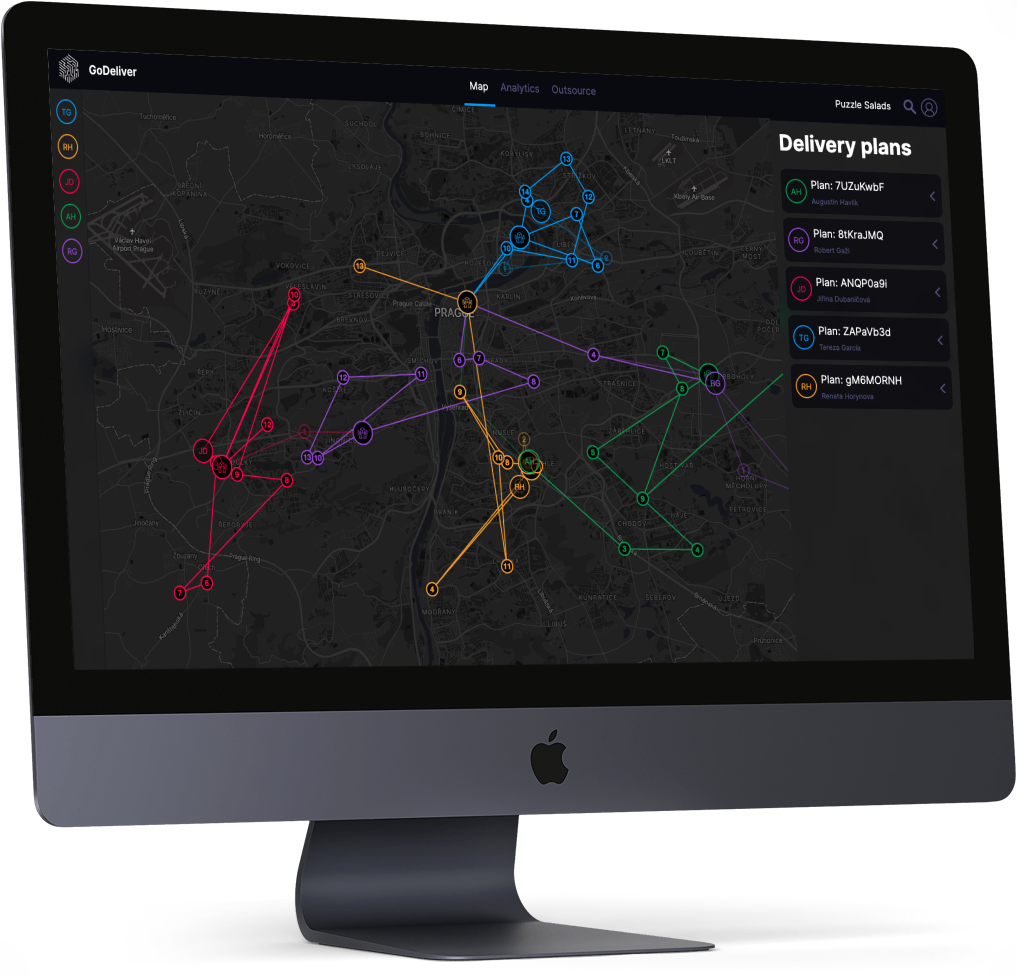
\includegraphics[width=0.5\textwidth]{resources/intro/godeliver-dashboard.png}
        \caption{GoDeliver dashboard visualizing solution for an instance of vehicle routing problem with time windows.}
        \label{fig:godeliver_dashboard}
    \end{figure}
    
    \section{Motivation}
    The paradigm shift in logistics business models towards instant gratification of customers are pushing the planning systems to be flexible and dynamic. The environment is constantly changing and planning systems have to update or entirely replan the instance in a short amount of time but maintaining the best delivery efficiency. Having a powerful planning system results in a dramatic reduction of delivery expanses.
    
    \section{Challenges}
    In the real world, the general VRP problem is not enough to solve the business-related problems. \gls{vrp} has multiple variants adding various constraints such as capacity, demand or time windows for given set of customers. The \gls{vrptw} is main focus of this thesis and we will be looking at some novel approaches how to solve it with \gls{ai}.
    
    \section{Assumptions} 
    We expect that leveraging \gls{ai} or \gls{ml} techniques to solve \gls{vrp} would lead in a drastic reduction of computational time for solving given instance of \gls{vrp}. Moreover, the time complexity would not be exponentially increasing with the problem size. The trade-off lays in the required time to allow \gls{ai} to train and learn how to solve the problem of vehicle routing.
    
    \section{Thesis structure}
    The rest of this thesis is organized as follows:
    \begin{itemize}
        \item Chapter \ref{introduction_vrp} presents an formal introduction to Vehicle Routing Problem.
        \item Chapter \ref{theoretical_background} provides an advanced theoretical background.
        \item Chapter 3 describes state-of-the-art solutions in optimization heuristics for solving \gls{vrptw}
        \item Chapter 4 describes state-of-the-art solutions in optimization heuristics for solving \gls{vrptw}
        \item Chapter 5 descImplementation details are explained in
        \item Chapter 6 summarizes our work, and presents possible future extensions.
    \end{itemize}
\end{introduction}